\subsection{Pad$\acute{e}$ Approximations}

\frame{
\begin{itemize}
\item In this section we introduce the notion of rational approximations for functions. 
\item The function $f(x)$ will be approximated over a small portion of its domain. 
\item For example, if $f(x) = cos(x)$, it is sufficient to have a formula to generate approximations on the interval $[0,\pi \slash 2]$. 
\item Then trigonometric identities can be used to compute $cos (x)$ for any value $x$ that lies outside $[0, \pi \slash 2]$. 
\end{itemize}
}

\frame{
A rational approximation to $f(x)$ on $[a, b]$ is the quotient of two polynomials $P_N(x)$ and $Q_M(x)$ of degrees $N$ and $M$, respectively.  
\begin{block}{ We use the notation $R_{N,M}(x)$ to denote  this quotient: }
\begin{equation*}
R_{N,M} (x) = \frac{P_N (x)}{Q_M(x)}  \ \ \ for \ \  a \le x \le b.
\end{equation*} 
\end{block}
Our goal is to {\huge make the maximum error as small as possible}.  \\
For a given amount of computational effort, one can usually construct a rational approximation that has a smaller overall error on $[a, b]$ than a polynomial approximation.  \\
Our development is an introduction and will be limited to Pad$\acute{e}$ approximations. 
}

\frame{
\begin{block}{The method of Pad$\acute{e}$ requires that $f(x)$ and its derivative be continuous at $x = 0$.}  
There are two reasons for the arbitrary choice of $x = 0$. 
\begin{itemize}
\item First, it makes the manipulations simpler. 
\item Second, a change of variable can be used to shift the calculations over to an interval that contains zero. 
\end{itemize}
\end{block}
The polynomials used in (3.101) are 
\begin{equation*}
P_N (x) = p_0 + p_1 x + p_2 x^2 + \cdots + p_N x^N
\end{equation*} 
and
\begin{equation*}
Q_M (x) = 1 + q_1 x + q_2 x^2 + \cdots +q_M x^M
\end{equation*} 
}

\frame{
\begin{itemize}
\item The polynomials $P_N(x)$ and $Q_N(x)$ are constructed so that $f(x)$ and $R_{N,M}(x)$ agree at $x = 0$ and their derivatives up to $N + M$ agree at $x = 0$. 
\item In the case $Q_0(x) = 1$, the approximation is just the Maclaurin expansion for $f (x)$. 
\item For a fixed value of $N + M$ the error is smallest when $P_N(x)$ and $Q_M(x)$ have the same degree or when $P_N(x)$ has degree one higher than $Q_M (x)$. 
\end{itemize}
}

\frame{
Notice that the constant coefficient of $Q_M$ is $q_0 = 1$. 
This is permissible, because it cannot be $0$ and $R_{N,M}(x)$ is not changed when both $P_N(x)$ and $Q_M(x)$ are divided by the same constant. 
Hence the rational function $R_{N,M}(x)$ has $N + M + 1$ unknown coefficients. 
Assume that $f(x)$ is analytic and has the Maclaurin expansion 
\begin{equation*}
f (x) = a_0 + a_1 x + a_2 x^2 + \cdots + a_k x^k + \cdots ,
\end{equation*}
and form the difference $f(x) Q_M(x) - P_N(x) = Z(x)$: 
\begin{equation*}
\left( \sum_{j=0}^\infty a_j x^j \right) \left( \sum_{j=0}^M q_j x^j \right)  - \sum_{j=0}^N p_j x^j= \sum_{j=N+M+1}^\infty c_j x^j
\end{equation*} 
The lower index $j = M +N + 1$ in the summation on the right side of (3.105) is chosen because the first $N + M$ derivatives of $f(x)$ and $R_{N,M}(x)$ are to agree at $x = 0$. 
}

\frame{
When the left side of (3.105) is multiplied out and the coefficients of the powers of $x^j$ are set equal to zero for $k = 0,1, ... , N + M$, the result is a system of $N + M + 1$ linear equations: 
\begin{equation*}
\begin{array}{r c l}
a_0 - p_0 & = & 0 \\
q_1 a_0 + a_1 - p_1 & = & 0 \\
q_2 a_0 + q_1 a_1 + a_2 - p_2 & = & 0 \\
q_3 a_0 + q_2 a_1 + q_1 a_2 + a_3 - p_3 & = & 0 \\
q_M a_{N-M} + q_{M-1}a_{N-M+1} + \cdots + a_N - p_N & = & 0
\end{array}
\end{equation*} 
and
\begin{equation*}
\begin{array}{r c r c c c r c r c c}
q_M a_{N-M+1} & + & q_{M-1} a_{N-M+2} & + & \cdots & + & q_1 a_N & + & a_{N+1} & = & 0 \\
q_{M} a_{N-M+2} & + & q_{M-1} a_{N-M+3} & + & \cdots & + & q_1 a_{N+1} & + & a_{N+2} & = & 0 \\
\vdots & & & & & & & & &  \vdots &  \\
q_M a_N & + & q_{M-1} a_{N+1} & + & \cdots & + & q_1 a_{N+M-1} & + & a_{N+M} & = & 0
\end{array}
\end{equation*} 
}

\frame{
\begin{itemize}
\item Notice that in each equation the sum of the subscripts on the factors of each product is the same, and this sum increases consecutively from $0$ to $N + M$. 
\item The $M$ equations in (3.107) involve only the unknowns $q_1$, $q_2$, $\ldots$, $q_M$ and must be solved first. 
\item Then the equations in (3.106) are used successively to find $p_1$, $p_2$, $\ldots$, $p_N$. 
\end{itemize}
}

\frame{
\frametitle{Example 3.17.} 
Establish the Pad$\acute{e}$ approximation
\begin{equation*}
\cos (x) \approx R_{4,4} (x) =\frac{ 15,120 - 6900x^2 + 313x^4}{15,120 + 660x^2 + 13x^4}
\end{equation*}
See thefollowing figure for the graphs of $\cos(x)$ and $R_{4,4}(x)$ over $[-5, 5]$.
\begin{figure}
\begin{center}
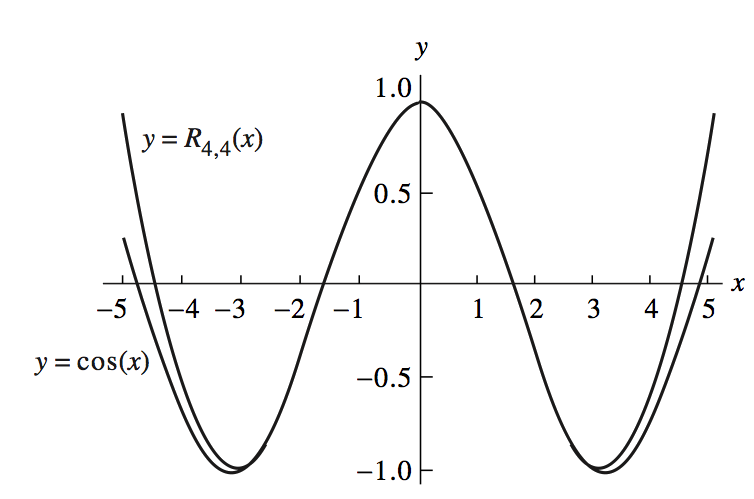
\includegraphics[width=70mm]{chap-3/fig_4-18.png}
\end{center}
\end{figure} 
}

\frame{
If the Maclaurin expansion for $cos(x)$ is used, we will obtain nine equations in nine unknowns. 
Instead, notice that both $cos (x)$ and $R_{4,4}(x)$ are even functions and involve powers of $x^2$. 
We can simplify the computations if we start with $f(x) = cos(x^{1 \slash2 })$: 
\begin{equation*}
f (x) = 1 - \frac{1}{2} x + \frac{1}{24} x^2 - \frac{1}{720} x^3 + \frac{1}{40,320} x^4 - \cdots .
\end{equation*} 
In this case, equation (3.105) becomes 
\begin{equation*}
\begin{array}{r}
\left( 1 - \frac{1}{2} x + \frac{1}{24} x^2 -\frac{1}{720} x^3 + \frac{1}{40,320} x^4 - \cdots \right)
\left( 1 + q+1 x + q_2 x^2 \right) - p_0 - p_1 x - p_2 x^2 \\
 = 0 + 0 x + 0 x^2 + 0 x^3 + 0 x^4 + c_5 x^5 + c_6 x^6 + \cdots
\end{array}
\end{equation*}
}

\frame{
When the coefficients of the first five powers of $x$ are compared, we get the following system of linear equations:
\begin{equation*}
\begin{array}{r c c}
1 - p_0 & = & 0 \\
-\frac{1}{2} + q_1 - p_1 & = & 0 \\
\frac{1}{24} - \frac{1}{2} q_1 + q_2 - p_2 & = & 0 \\
-\frac{1}{720} + \frac{1}{24} q_1 - \frac{1}{2} q_2 & = & 0 \\
\frac{1}{40,320} - \frac{1}{720} q_1 + \frac{1}{24} q_2 & = & 0
\end{array}
\end{equation*}
%\begin{figure}
%\begin{center}
%\includegraphics[width=60mm]{fig/ch-3/eq_3-110.png}
%\end{center}
%\end{figure} 
The last two equations in (3.110) must be solved first. 
They can be rewritten in a form that  is easy to solve: 
\begin{equation*}
q_1 - 12 q_2 =\frac{1}{30} \ \ \ and \ \ \ - q_1 + 30 q_2 = -\frac{1}{56}
\end{equation*}
}

\frame{
First find $q_2$ by adding the equations; then find $q_1$:
\begin{equation*}
q_2 = \frac{1}{18} \left( \frac{1}{30} - \frac{1}{56} \right) = \frac{13}{15,120}
\end{equation*} 
\begin{equation*}
q_1 = \frac{1}{30} + \frac{156}{15,120} = \frac{11}{252}
\end{equation*} 
}

\frame{
Now the first three equations of (3.110) are used. 
\begin{block}{
It is obvious that $p_0 = 1$, and we can use $q_1$ and $q_2$ in (3.111) to solve for $p_1$ and $p_2$:}
\begin{equation*}
p_1 = -\frac{1}{2} + \frac{11}{252} = -\frac{115}{252}
\end{equation*} 
\begin{equation*}
p_2 = \frac{1}{24} - \frac{11}{504} + \frac{13}{15,120} = \frac{313}{15,120}
\end{equation*} 
\end{block}
}

\frame{
\begin{block}{
Now use the coefficients in (3.111) and (3.112) to form the rational approximation to $f(x)$: }
\begin{equation*}
f(x) \approx \frac{1 - 115 x \slash 252 + 313 x^2 \slash 15,120}{1 + 11x \slash 252 + 13x^2 \slash 15,120}
\end{equation*} 
\end{block}
Since $cos(x) = f(x^2)$, we can substitute $x^2$ for $x$ in equation (3.113) and the result is the formula for $R_{4,4}(x)$ in (3.108). 
}


